En esta sección se realizaron pruebas para verificar el funcionamiento de todos los módulos del sistema embebido y la aplicación móvil.

\section{Cálculo de frecuencia cardíaca}

\subsection{Prueba unitaria}
Para verificar que el módulo tenga un correcto funcionamiento, se probó de manera unitaria conectándolo directamente a la computadora a través de la interfaz USB del módulo.\\ %La conexión entra ambos componentes se realizó de forma cruzada, es decir, que el transmisor de un dispositivo fue conectado al receptor del otro, tal como se muestra en la figura \ref{fig:ConexionUART}.
%
%	\begin{figure}[htbp!]
%		\centering
%		\fbox{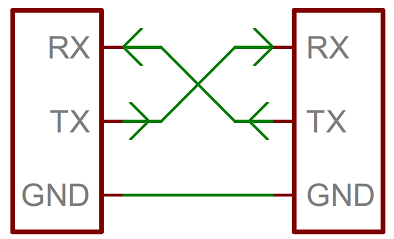
\includegraphics[width=0.4\textwidth]{AvancesPruebas/imagenes/conexion-uart.png}}
%		\caption{Conexión UART de módulo GSM y FT232}
%		\label{fig:ConexionUART}
%	\end{figure}
	
Una vez conectado correctamente ambos componentes, se realizó la prueba de la siguiente forma:
\begin{enumerate}
	\item Se ejecutó el emulador de terminal ’PuTTY’, configurándolo para el puerto serial
	indicado, con un baudaje de 19200, transmisión de 8 bits, sin paridad con 1 bit de
	stop y sin flujo de control. La configuración realizada se muestra en la figura \ref{fig:ConfiguracionPutty}.
	\item Se ejecutaron los comandos AT básicos para probar el módulo LARA-R202 y se confirmó que en ninguno de ellos se mostrará un error. Algunos de los comandos utilizados, son:

		\begin{enumerate}
			\item AT
			\item AT+ATE0
			\item AT+CMGF=1
			\item AT+CMGS=""
		\end{enumerate}	
\end{enumerate}
 
	\begin{figure}[htbp!]
		\centering
		\fbox{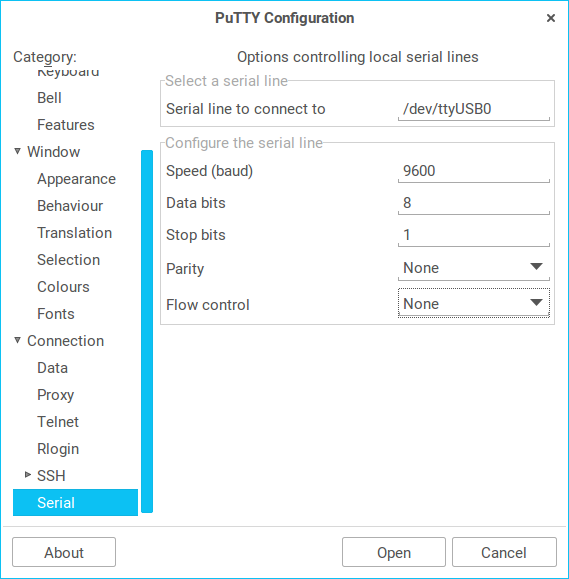
\includegraphics[width=0.7\textwidth]{AvancesPruebas/imagenes/putty.png}}
		\caption{Configuración de terminal en PuTTY}
		\label{fig:ConfiguracionPutty}
	\end{figure}
 
El resultado de los comandos ejecutados mediante la terminal de PuTTY se muestra en la figura \ref{fig:TerminalPutty}.

	\begin{figure}[htbp!]
		\centering
		\fbox{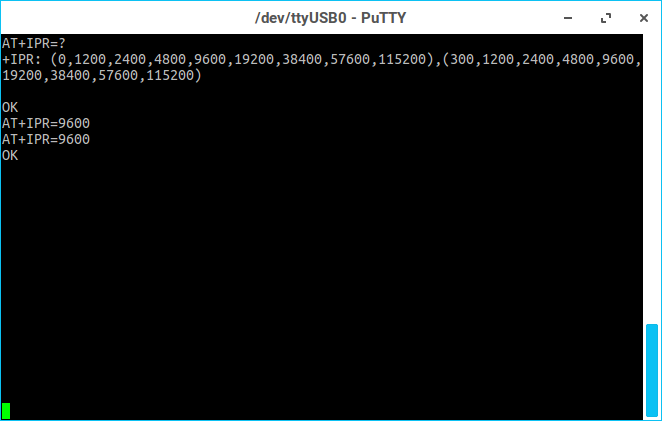
\includegraphics[width=0.7\textwidth]{AvancesPruebas/imagenes/putty_ipr.png}}
		\caption{Comandos AT en terminal de PuTTY}
		\label{fig:TerminalPutty}
	\end{figure}


\subsection{Conexión con microcontrolador}
Después de asegurar el funcionamiento del módulo 4G, se realizó el programa correspondiente para la comunicación con el microcontrolador.\\

La conexión fue realizada mediante el UART2 del microcontrolador y mediante comandos AT se creó la rutina para verificar el envío de un mensaje SMS a un número de teléfono específico.\\

El proceso para establecer la comunicación del módulo GSM con el dsPIC y la computadora fue el siguiente.\\

Como primer paso se inicializaron los periféricos del dsPIC necesarios para la comunicación, en este caso fue el UART1 para transmitir a la pc los resultado obtenidos, el UART2 para la comunicación con el módulo 4G y las entradas y salidas del mikrobus2 que necesita el módulo para funcionar correctamente. \\

La conexión del módulo 4G se realizó mediante un Mikrobus conectado al microcontrolador. El esquema de esta conexión, así como la conexión física se muestran en las figuras \ref{fig:ConexionAD8232} y \ref{fig:ConexionFisicaGSM} respectivamente.

	\begin{figure}[htbp!]
		\centering
		\fbox{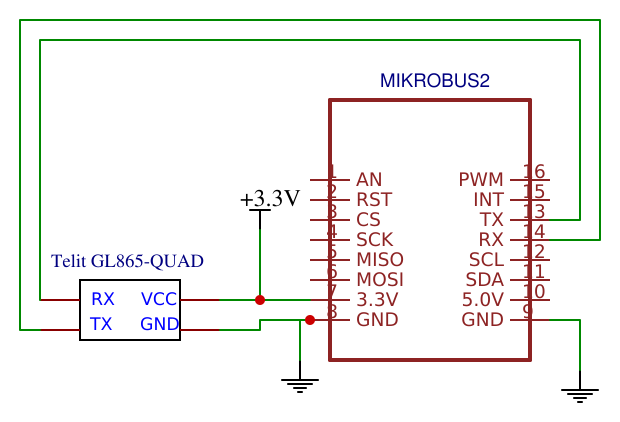
\includegraphics[width=0.7\textwidth]{AvancesPruebas/imagenes/GSMConexion.png}}
		\caption{Conexión del módulo 4G con microcontrolador}
		\label{fig:ConexionGSM}
	\end{figure}
	
	\begin{figure}[htbp!]
		\centering
		\fbox{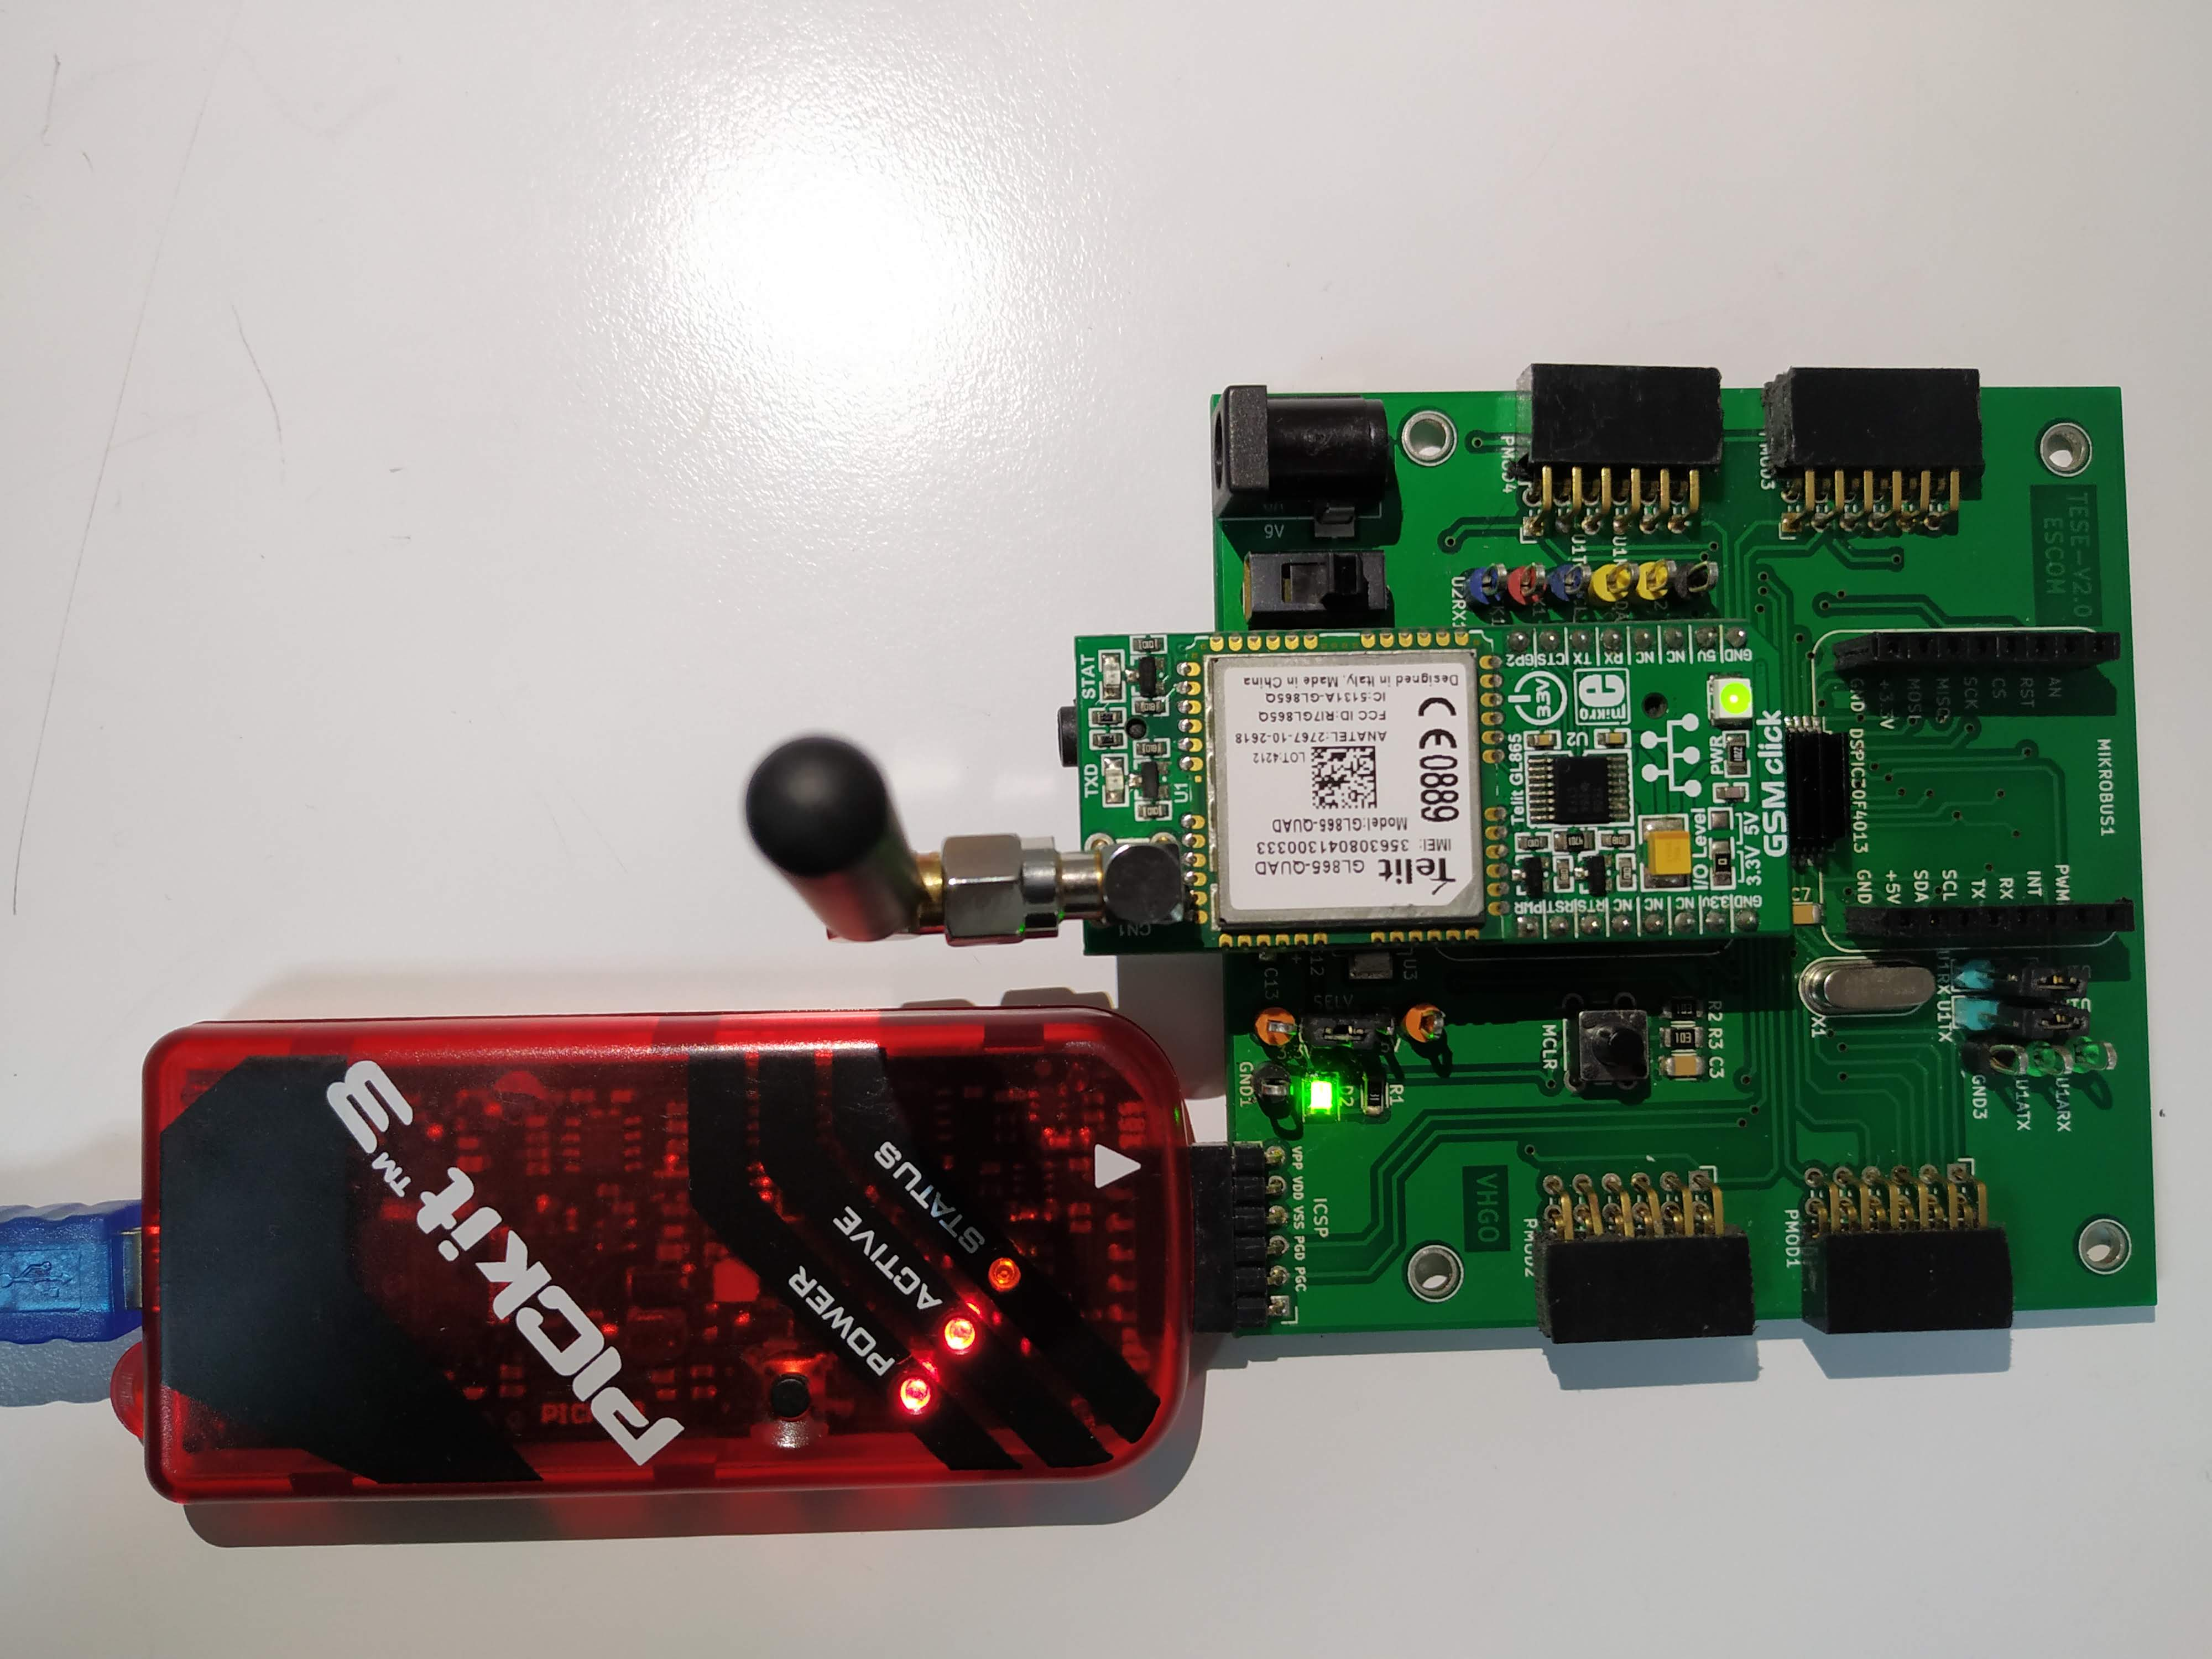
\includegraphics[width=0.7\textwidth]{AvancesPruebas/imagenes/ConexionFisicaGSM.jpg}}
		\caption{Conexión física del módulo 4G con microcontrolador mediante Mikrobus2}
		\label{fig:ConexionFisicaGSM}
	\end{figure}
	
En la figura \ref{fig:RecepcionMsj} se muestra la captura de pantalla que contiene el mensaje recibido en el teléfono celular.

	\begin{figure}[htbp!]
		\centering
		\fbox{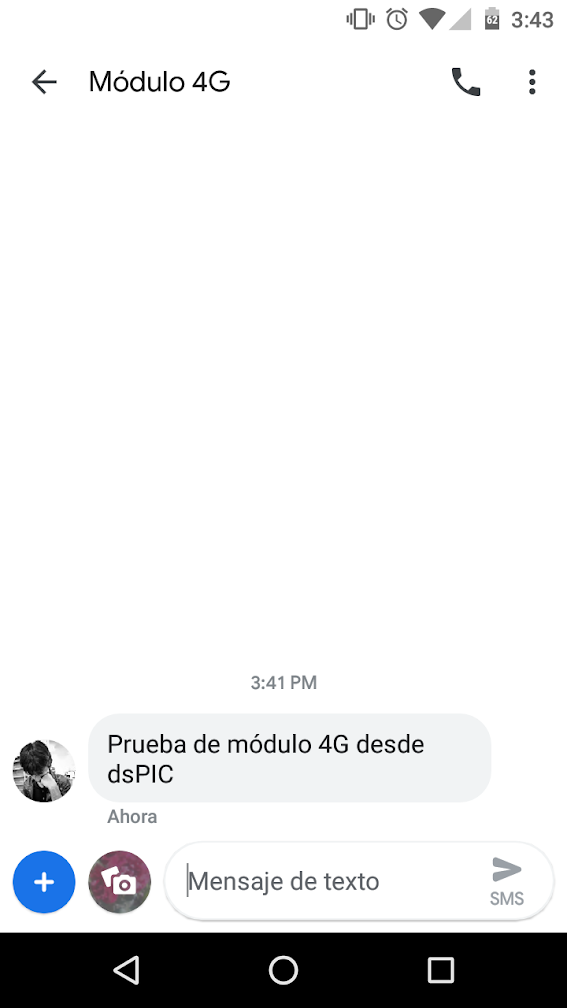
\includegraphics[width=0.35\textwidth]{AvancesPruebas/imagenes/msjModulo.png}}
		\caption{Recepción de mensaje enviado por el módulo 4G}
		\label{fig:RecepcionMsj}
	\end{figure}
	
	\clearpage
